\scanpage{416}

Composition with the canonical projection to
$T_\rho\times N'_\sigma$ gives a \uline{monomorphism}

\margin{for we shall have
\diagram{\begin{tikzcd}[ampersand replacement=\&]
T_0 \arrow[r,"{\substack{\det\\\sim}}"] \& \mathbb G_m
\end{tikzcd}}}

\[
(24)\qquad
\diagram{\begin{tikzcd}[ampersand replacement=\&,column sep=large]
\mathcal T_{\rho,\sigma} \arrow[r,hook] \arrow[d,phantom,"{\rotatebox{90}{$\simeq$}}" description]
 \& T_\rho\times N'_\sigma \\
\left\{(\underline a,\underline b)\mid
 (\det\underline a/\det\underline b)^2=1\right\}
 \& \inserted{\left.\begin{gathered}
\text{i.e. }\det\underline a=\varepsilon'\det\underline b\\
\text{with }\varepsilon'^2=1
\end{gathered}\right\}}
\end{tikzcd}}
\]

and we shall therefore have
\[
(25)\qquad
\left\{\begin{aligned}
\chi(\underline a,\underline b)&=\det\underline b\\
\varepsilon_2(\underline a,\underline b)&=\varepsilon_\sigma(\underline b)\\
\varepsilon_3(\underline a,\underline b)&=\det(\underline a)/\det(\underline b)
 =\det\underline b/\det\underline a
\end{aligned}\right.
\]

We define
\[
(26)\qquad
\diagram{\begin{tikzcd}[ampersand replacement=\&,column sep=small]
\mathcal T_{\rho,\sigma}^{\circ} \arrow[d,phantom,"{\rotatebox{90}{$\simeq$}}" description]
 \& {}=\operatorname{Ker}\mathcal T_{\rho,\sigma}
 \arrow[r,"{(\varepsilon_2,\varepsilon_3)}"]
 \& \mu_2\times\mu_2 \\
\inserted{T_\rho\times_{\mathbb G_m}T_\sigma} \&\&
\end{tikzcd}}
\]
so we have
\[
(27)\qquad
\diagram{\begin{tikzcd}[ampersand replacement=\&]
1 \arrow[r] \& \mathcal T_{\rho,\sigma}^{\circ} \arrow[r]
 \& \mathcal T_{\rho,\sigma} \arrow[r] \& \mu_2\times\mu_2 \arrow[r] \& 1
\end{tikzcd}}
\]
and a canonical exact sequence
\[
(28)\qquad
\diagram{\begin{tikzcd}[ampersand replacement=\&]
1 \arrow[r] \&
\overbrace{ST_\rho\times ST_\sigma}^{\inserted{\mathcal T_{\rho,\sigma}^{\circ+}}}
\arrow[r] \& \mathcal T_{\rho,\sigma}^{\circ} \arrow[r,"{\chi}"]
 \& \mathbb G_m \arrow[r] \& 1,
\end{tikzcd}}
\]
where we define
\[
(29)\qquad
\left\{\begin{aligned}
ST_\rho&=\{g\in\Gamma T_\rho\mid\det g=1\}\\
ST_\sigma&=\{g\in\Gamma T_\sigma\mid\det g=1\}
\end{aligned}\right.\quad.
\]

\margin{\figure{\begin{tikzpicture}[x=.65cm,y=.65cm]
\draw[->] (0,4.5) .. controls (1.1,4.55) and (1.1,3.7) .. (1.1,3.25)
 -- (1.2,.8) .. controls (1.2,.45) and (1.55,.55) .. (2.4,.65);
\draw (0,0) .. controls (1.0,-.05) and (1.05,.1) .. (1.15,.45)
 .. controls (1.25,.75) and (1.55,.65) .. (2.4,.65);
\end{tikzpicture}}}
\inserted{The operation of $\mathcal T_{\rho,\sigma}\simeq
\mathcal M_{\rho,\sigma}(0)$ on $L_0$ is given by
\[
(30)\qquad g(\varepsilon_0(\lambda))=\varepsilon_0(\mu\lambda),
\quad\text{where }\mu=\chi(g)
\]}

We let $\mathcal M_{\rho,\sigma}(0)
(\simeq\mathcal T_{\rho,\sigma})$ operate on $SG$, by
\[
(31)\qquad
\diagram{\begin{tikzcd}[ampersand replacement=\&,column sep=large]
\mathcal M_{\rho,\sigma}(0)
 \arrow[r,"{\text{projection}}"]
 \& T_0 \arrow[r,"{\substack{\text{canonical}\\(\text{monomorphism})}}"]
 \& PG \arrow[r,"{\sim}"]
 \& \underline{\operatorname{Aut}}_{\mathrm{gr}}(SG) \\
T_0\times T_\rho\times N'_\sigma \arrow[u,phantom,"{\cap}" description]
 \& G \arrow[u,phantom,"{\cap}" description]
 \& G/\mathbb G_m\simeq\underline{\operatorname{Aut}}(G)
 \arrow[u,phantom,"{\rotatebox{90}{$\simeq$}}" description] \&
\end{tikzcd}}
\]

\par\noindent 415

\scanpage{417}
\mspage{510}

and we define
\[
(32)\qquad \mathcal M_{\rho,\sigma}\simeq
 \mathcal M_{\rho,\sigma}(0)\mathbin{.}SG
\]
\hfill $\frac12$ direct product

We thus have a canonical homomorphism
\[
(33)\qquad
\diagram{\begin{tikzcd}[ampersand replacement=\&]
SG \arrow[r,hook,"{j}"] \& \mathcal M_{\rho,\sigma}
\end{tikzcd}}
\]
whose image is denoted $\widetilde{\mathcal G}_{\rho,\sigma}^{+}$, so
\[
(34)\qquad
\diagram{\begin{tikzcd}[ampersand replacement=\&]
1 \arrow[r] \& \widetilde{\mathcal G}_{\rho,\sigma}^{+} \arrow[r]
 \& \mathcal M_{\rho,\sigma} \arrow[r] \& \mathcal T_{\rho,\sigma} \arrow[r] \& 1
\end{tikzcd}}
\]
\[
(35)\qquad
\diagram{\begin{tikzcd}[ampersand replacement=\&,column sep=0.3em,row sep=1.3em]
\mathcal M_{\rho,\sigma}\simeq \& \mathcal M_{\rho,\sigma}(0)
 \arrow[d,phantom,"{\rotatebox{90}{$\simeq$}}" description]
 \& {}\mathbin{.}\widetilde{\mathcal G}_{\rho,\sigma}^{+} \\
 \& \mathcal T_{\rho,\sigma} \&
\end{tikzcd}}
\]
\hfill $\frac12$ direct product.

\uline{N.B.} We use the notation $\mathcal T_{\rho,\sigma}$ for the
quotient group
\[
(36)\qquad \mathcal T_{\rho,\sigma}\simeq
\mathcal M_{\rho,\sigma}/\widetilde{\mathcal G}_{\rho,\sigma}^{+},
\]
the notation $\mathcal M_{\rho,\sigma}[0)$ for the subgroup
of $\mathcal M_{\rho,\sigma}$.

We define a canonical embedding
\[
(37)\qquad
\diagram{\begin{tikzcd}[ampersand replacement=\&]
\mathcal M_{\rho,\sigma}[0] \arrow[r,hook,"{i}"] \& \mathcal M_{\rho,\sigma}
\end{tikzcd}}
\]
which extends the inclusions \unsure{of the subgroups|of the subgroup}
$\mathcal M_{\rho,\sigma}(0)$ common to $\mathcal M_{\rho,\sigma}[0]$
and to $\mathcal M_{\rho,\sigma}$,
and which on $L_0$ is given by
\[
(38)\qquad i(\lambda)=j(\lambda)\qquad (\text{cf. }(33))
\]
(which is indeed compatible with the operations of
$\deleted{\unsure{\mathcal T|\mathcal M}}\mathcal M_{\rho,\sigma}(0)$
on $L_0$ on the one hand, on $SG\simeq\widetilde{\mathcal G}_{\rho,\sigma}^{+}$
on the other).

\par\noindent 416

\scanpage{418}

Another way of saying it is to observe that
$\mathcal M_{\rho,\sigma}(0)$ operating on
$SG\simeq\widetilde{\mathcal G}_{\rho,\sigma}^{+}$
normalizes the subgroup $j(L_0)$ -- which we
henceforth identify with $L_0$), so that we
shall have a subgroup
\[
\mathcal M_{\rho,\sigma}(0)\mathbin{.}L_0\subset\mathcal M_{\rho,\sigma}
\]
which \unsure{is|will be} canonically isomorphic to $\mathcal M_{\rho,\sigma}[0]$
defined above, thanks to the expression $(\unsure{19|49})$ of
the latter as a $\frac12$-direct product.

\deleted{\uline{Proposition}}
\inserted{\uline{Remark.}} We have
\[
\deleted{(\unsure{39})}\qquad
\mathcal M_{\rho,\sigma}[0]\subset
\underline{\operatorname{Norm}}_{\mathcal M_{\rho,\sigma}}(L_0)
\]

By construction, \deleted{\unsure{we have} $\subset$, \unsure{for} $\unsure{\supset}$}
the inclusion in the reverse direction would amount to saying that $L_0$
is its own normalizer in $SG\simeq\widetilde{\mathcal G}_{\rho,\sigma}^{+}$,
which of course is not true at all
-- \unsure{even} though the analogous fact is true
in the profinite group
$\widetilde{\mathcal G}_{0,3}^{\widehat{+}}$,
for the subgroup generated by $\varepsilon_0$,
or in $\Pi_{0,\widehat{3}}$ for
the one generated by $l_0$ (\unsure{subject to} verification !
besides which I still haven't done).

\par\noindent 417

\scanpage{419}
\mspage{511}

\margin{$\mathcal M_{\rho,\sigma}^{\circ},\mathcal M_{\rho,\sigma}^{+},
\mathcal M_{\rho,\sigma}^{+\circ},\mathcal T_{\rho,\sigma}^{\circ},
\mathcal T_{\rho,\sigma}^{+},\mathcal T_{\rho,\sigma}^{\circ+}\ldots$
some central subgroups and computations of integral \unsure{points}\ldots}

\Needspace{14\baselineskip}
\figure{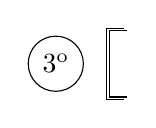
\begin{tikzpicture}[baseline=(n.base)]
\node[draw,circle,inner sep=3pt] (n) at (0,0) {$3^{\mathrm o}$};
\draw[line width=.6pt] (.90,.42)--(.68,.42)--(.68,-.42)--(.90,-.42);
\draw[line width=.45pt] (.86,.45)--(.64,.45)--(.64,-.45)--(.86,-.45);
\end{tikzpicture}}\par\nobreak
We denote by $\mathcal M_{\rho,\sigma}^{\circ}$,
$\mathcal M_{\rho,\sigma}[0]^{\circ}$,
$\deleted{\unsure{\mathcal M}}\mathcal M_{\rho,\sigma}[0)^{\circ}$
identity components, we shall have for example
\[
(39)\qquad
\diagram{\begin{tikzcd}[ampersand replacement=\&,column sep=small]
1 \arrow[r] \& \mathcal M_{\rho,\sigma}^{\circ}
 \arrow[r] \arrow[d,phantom,"{\rotatebox{90}{$\simeq$}}" description]
 \& \mathcal M_{\rho,\sigma} \arrow[r] \& \mu_2\times\mu_2 \arrow[r] \& 1\\
 \& \mathcal M_{\rho,\sigma}^{\circ}(0)\mathbin{.}\widetilde{\mathcal G}_{\rho,\sigma}^{+}
 \&\&\&
\end{tikzcd}}
\]
\hspace*{4em} $\frac12$ direct product
\[
(40)\qquad
\diagram{\begin{tikzcd}[ampersand replacement=\&]
\mathcal M_{\rho,\sigma}(0)^{\circ} \arrow[r,"{\sim}"]
 \& \mathcal T_{\rho,\sigma}^{\circ}\simeq T_\rho\times_{\mathbb G_m}T_\sigma
\end{tikzcd}}
\]
\[
(41)\qquad
\begin{gathered}
\mathcal M_{\rho,\sigma}^{\circ}\text{ is the inverse image of }
\mathcal T_{\rho,\sigma}^{\circ}\\
\text{under }\diagram{\begin{tikzcd}[ampersand replacement=\&]
\mathcal M_{\rho,\sigma} \arrow[r,"{\text{canonical}}"] \& \mathcal T_{\rho,\sigma}
\end{tikzcd}},
\end{gathered}
\]

we have a canonical composite homomorphism
\[
(42)\qquad
\diagram{\begin{tikzcd}[ampersand replacement=\&]
\mathcal M_{\rho,\sigma} \arrow[r] \& \mathcal T_{\rho,\sigma}
 \arrow[r,"{\chi}"] \& \mathbb G_m
\end{tikzcd}}
\]
also denoted $\chi$, its kernel is denoted
$\mathcal M_{\rho,\sigma}^{+}$, and we define in the $=$ way
$\mathcal M_{\rho,\sigma}^{\circ+}$, so
\[
(43)\qquad
\diagram{\begin{tikzcd}[ampersand replacement=\&]
1 \arrow[r] \& \mathcal M_{\rho,\sigma}^{+} \arrow[r]
 \arrow[d,phantom,"{\unsure{\cup|\downarrow}}" description]
 \& \mathcal M_{\rho,\sigma} \arrow[r,"{\chi}"]
 \arrow[d,phantom,"{\unsure{\cup|\downarrow}}" description]
 \& \mathbb G_m \arrow[r]
 \arrow[d,phantom,"{\unsure{\cup|\downarrow}}" description] \& 1\\
1 \arrow[r] \& \mathcal M_{\rho,\sigma}^{\circ+} \arrow[r]
 \& \mathcal M_{\rho,\sigma}^{\circ} \arrow[r,"{\chi}"]
 \& \mathbb G_m \arrow[r] \& 1
\end{tikzcd}}
\]
\[
(44)\qquad
\left\{\begin{aligned}
\mathcal M_{\rho,\sigma}^{+}&\simeq
\underbrace{\mathcal M_{\rho,\sigma}^{+}(0)}_{
\substack{\rotatebox{90}{$\simeq$}\\\mathcal T_{\rho,\sigma}^{+}}}
\mathbin{.}\widetilde{\mathcal G}_{\rho,\sigma}^{+}\\[3em]
\mathcal M_{\rho,\sigma}^{\circ+}&\simeq
\underbrace{\mathcal M_{\rho,\sigma}^{\circ+}(0)}_{
\substack{\rotatebox{90}{$\simeq$}\\
\mathcal T_{\rho,\sigma}^{\circ+}\simeq ST_\rho\times ST_\sigma\\
\text{cf. }(28)}}
\mathbin{.}\widetilde{\mathcal G}_{\rho,\sigma}^{+}
\end{aligned}\right.
\]

Thus we have
\[
(45)\qquad
\begin{gathered}
\mathcal M_{\rho,\sigma}^{\circ+}(0)\overset{\mathrm{dfn}}=
\operatorname{Ker}\left(\diagram{\begin{tikzcd}[ampersand replacement=\&]
\mathcal M_{\rho,\sigma}^{\circ}(0)
 \arrow[r,"{{\chi,\varepsilon_2,\varepsilon_3}}"]
 \& \mathbb G_m\times\mu_2\times\mu_2
\end{tikzcd}}\right)\\
\simeq ST_\rho\times ST_\sigma
\end{gathered}
\]
and this subgroup is \uline{central} in
$\mathcal M_{\rho,\sigma}^{\circ}$
(not in $\mathcal M_{\rho,\sigma}$), more precisely

\par\noindent 418

\scanpage{420}

we have
\[
\begin{aligned}
(46)\qquad
\mathcal M_{\rho,\sigma}^{\circ+}
&\overset{\mathrm{dfn}}{=}
\operatorname{Ker}\bigl(\mathcal M_{\rho,\sigma}
\xrightarrow{(\chi,\varepsilon_2,\varepsilon_3)}
\mathbb G_m\times\mu_2\times\mu_2\bigr)
\deleted{\unsure{\simeq}}\\
&\simeq
\underbrace{ST_\rho\times ST_\sigma}_{\subset\mathcal M_{\rho,\sigma}(0)}
\times\widetilde{\mathcal G}_{\rho,\sigma}^{+}
\end{aligned}
\]

\margin{The whole end of the number should come
after (or before) \unsure{the} number $6^\circ$
\unsure{about} the ``\unsure{radicalities}''}

\margin{$\circ$ Careful, this inclusion is not an equality,
cf. below\ldots}

\[
(47)\qquad
\uline{\operatorname{Centr}}(\mathcal M_{\rho,\sigma}^{\circ})
\supset
\underbrace{1\times ST_\rho\times ST_\sigma}_{\substack{\cap\\
\mathcal M_{\rho,\sigma}(0)^\circ}}
\times
\underset{\substack{\cap\\\widetilde{\mathcal G}_{\rho,\sigma}^{+}\simeq SG}}{\mu_2}.
\]

Hence a subgroup
\[
(48)\qquad
\mu_2\times\mu_2\times\mu_2
\subset 1\times
\underbrace{ST_\rho\times ST_\sigma\times\mu_2}_{\substack{\cap\\
\operatorname{Centr}(\mathcal M_{\rho,\sigma}^{\circ})}}
\]
which is in fact contained in the Center of $\mathcal M_{\rho,\sigma}$
as a whole, for
\[
(49)\qquad
\uline{\operatorname{Centr}}(\mathcal M_{\rho,\sigma})
\supset
\underbrace{1\times S'T_\rho\times\mu_2}_{\substack{\cap\\
\mathcal M_{\rho,\sigma}(0)}}
\times
\underset{\substack{\cap\\\widetilde{\mathcal G}_{\rho,\sigma}^{+}\simeq SG}}{\mu_2}
\]
\margin{\unsure{id.}}
with
\[
(50)\qquad
S'T_\rho\overset{\mathrm{dfn}}{=}
\{g\in\Gamma T_\rho\mid(\det g)^2=1\}
\]
so that we have
\diagram{\begin{tikzcd}[ampersand replacement=\&,column sep=large]
\text{(51)}\quad 1 \arrow[r] \& ST_\rho \arrow[r] \&
S'T_\rho \arrow[r,"{\varepsilon_3}"] \& \mu_2 \arrow[r] \& 1
\end{tikzcd}}

We thus have
\[
(52)\qquad
\operatorname{Centr}(\mathcal M_{\rho,\sigma})\cap
\mathcal M_{\rho,\sigma}^{\circ}
\supset
\underset{\substack{\cap\\T_0}}{1}\times
\underset{\substack{\cap\\T_\rho}}{ST_\rho}\times
\underset{\substack{\cap\\T_\sigma}}{\mu_2}\times
\underset{\substack{\cap\\\widetilde{\mathcal G}_{\rho,\sigma}^{+}}}{\mu_2}.
\]
\margin{\unsure{id.}}

The ``modular case'' is the one where
\[
(53)\qquad
\left\{\begin{aligned}
\det\rho&=1\quad\text{i.e.}\quad\det\sigma=1
\quad\text{i.e.}\quad\nu=-1\\
\text{i.e.}\quad\rho&=\begin{pmatrix}0&1\\-1&1\end{pmatrix}
\quad\text{i.e.}\quad\sigma=\begin{pmatrix}0&1\\-1&0\end{pmatrix}
\end{aligned}\right.
\]
(cf. \uline{$\overline{\mathrm{VI}}$} for other
characterizations, such as
$\sigma^2=-1$, or $\rho^2-\rho+1=0$, or
$\widetilde\sigma^2=\widetilde\rho^3=1\ldots$),
this also means that $\rho$ (as an element of $T_\rho$)
is in $ST_\rho$ hence in the \unsure{center} of $\mathcal M_{\rho,\sigma}^{\circ}$,

\par\noindent 419

\scanpage{421}
\mspage{512}

or that $\sigma$ as an element of $T_\sigma$
is in $ST_\sigma$ i.e. in the center of $\mathcal M_{\rho,\sigma}^{\circ}$.
So in this case we find a homomorphism
\diagram{\(\displaystyle
(54)\quad\left\{
\begin{gathered}
\begin{tikzcd}[ampersand replacement=\&,column sep=large,row sep=large]
\mathbb Z/6\mathbb Z\times\mathbb Z/4\mathbb Z \arrow[r] \&
\uline{\operatorname{Centr}}(\mathcal M_{\rho,\sigma}^{\circ})\\
(i,j) \arrow[r] \& i_\rho(\rho^i)i_\sigma(\sigma^j)
\end{tikzcd}
\end{gathered}\right.
\)}
(where we define $i_\rho,i_\sigma$ among the
\deleted{\unsure{four}}\inserted{three} canonical morphisms
\[
\deleted{(55)\quad\unsure{i_B}:B'_0\longrightarrow
\mathcal M_{\rho,\sigma}[0]\subset\mathcal M_{\rho,\sigma}}
\]
\diagram{\(\displaystyle
(55)\quad\left\{
\begin{gathered}
\begin{tikzcd}[ampersand replacement=\&,column sep=large,row sep=small]
i_\rho:S'T_\rho \arrow[r] \& \mathcal M_{\rho,\sigma}(0)
\arrow[r,phantom,"{\subset}" description] \& \mathcal M_{\rho,\sigma}\\
i_\sigma:\unsure{SN'_\sigma} \arrow[r] \& \mathcal M_{\rho,\sigma}(0)
\arrow[r,phantom,"{\subset}" description] \& \mathcal M_{\rho,\sigma}\\
i_G:SG\simeq\widetilde{\mathcal G}_{\rho,\sigma}^{+}
\arrow[r] \& \mathcal M_{\rho,\sigma}, \&
\end{tikzcd}
\end{gathered}\right.\qquad)
\)}
whose image, for $2$ invertible on $S$, contains
contains the image of $\mu_2\times\mu_2\times1$ in (48).
For $2$ invertible on $S$, the homomorphism (53) is a monomorphism
(but not in characteristic $2$, of course). Over the absolute base $\mathbb Z$,
we have moreover, in the modular case
\[
(56)\qquad
\left\{\begin{aligned}
\mathcal T_{\rho,\sigma}(\mathbb Z)&\simeq
T_\rho(\mathbb Z)\times N'_\sigma(\mathbb Z)
\simeq\mathbb Z/6\mathbb Z\times\mathbb D_4\\
\mathcal M_{\rho,\sigma}(\mathbb Z)&\simeq
\mathcal T_{\rho,\sigma}(\mathbb Z)\mathbin{.}\operatorname{Sl}(2,\mathbb Z)
\end{aligned}\right.
\]
\inserted{$\frac12$ direct product,
$\unsure{\mathbb D|\mathcal B|\mathcal T}_{\rho,\sigma}\simeq
\mathbb Z/6\mathbb Z\times\mathbb D_4$ operating via the character
\diagram{\begin{tikzcd}[ampersand replacement=\&,column sep=large]
\mathbb D_4 \arrow[r,"{\varepsilon_2}"] \&
\mathbb Z/2\mathbb Z\simeq\unsure{(1,\tau_\infty)|\{1,\tau_\infty\}}
\end{tikzcd}}
$\tau_\infty$ operating on $\operatorname{Sl}(2,\mathbb Z)$ by
automorphism induced by the matrix
\[
\tau_\infty=\begin{pmatrix}-1&0\\0&1\end{pmatrix}
\]
}

\margin{\figure{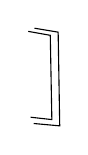
\begin{tikzpicture}[x=1cm,y=1cm]
\draw (0,1.15)--(.28,1.10)--(.30,.03)--(.03,.06);
\draw (.08,1.19)--(.38,1.14)--(.40,-.05)--(.07,-.02);
\end{tikzpicture}}}

\par\noindent 420

\scanpage{422}

\margin{the homomorphisms $\Theta,\widetilde\Theta$
$\Theta^\circ,\widetilde\Theta^\circ$}

\textcircled{\(4^\circ\)}\quad We define a homomorphism
\diagram{\begin{tikzcd}[ampersand replacement=\&,column sep=huge]
\text{(57)}\quad\mathcal M_{\rho,\sigma} \arrow[r,"{\Theta}"] \& G
\end{tikzcd}}
\[
\Theta\mid\widetilde{\mathcal G}_{\rho,\sigma}^{+}\simeq SG
\quad\text{is the identity}
\]
\[
\Theta\mid\mathcal M_{\rho,\sigma}(0)\subset
T_0\times T_\rho\times N'_\sigma
\quad\text{given by}\quad
\Theta(\underline u,\underline a,\underline b)=\underline u
\]
hence
\[
(58)\qquad
\Theta\mid\mathcal M_{\rho,\sigma}[0]\subset
B'_0\times T_\rho\times N'_\sigma
\quad\text{given by}\quad
\Theta(\underline u,\underline a,\underline b)=\underline u
\]

We have
\diagram{\begin{tikzcd}[ampersand replacement=\&,column sep=large,row sep=large,nodes in empty cells]
\text{(59)}\quad\deleted{\operatorname{Ker}\Theta=}
\arrow[d,phantom,"{\deleted{\simeq}}"{description,rotate=90}]
\& \mathcal M_{\rho,\sigma}(0)
\arrow[r,phantom,"{\subset}" description]
\arrow[d,phantom,"{\cup}" description]
\arrow[dr,phantom,"{\text{Cartesian}}" description]
\& T_0\times T_\rho\times N'_\sigma
\arrow[d,phantom,"{\cup}" description]\\
\deleted{\unsure{\mathcal R|SG}}
\& \operatorname{Ker}\Theta
\arrow[r,phantom,"{\subset}" description]
\& 1\times T_\rho\times N'_\sigma
\end{tikzcd}}
\[
\begin{gathered}
\rotatebox{90}{$\simeq$}\quad
\left\{\left(1,
\underset{\substack{\rotatebox{90}{$\in$}\\\Gamma T_\rho}}{\underline a},
\underset{\substack{\rotatebox{90}{$\in$}\\\Gamma N'_\sigma}}{\underline b}
\right)\,\middle|\,\det\underline b=1,(\det\underline a)^2=1\right\}\\
\rotatebox{90}{$\simeq$}\quad S'T_\rho\times SN'_\sigma
\end{gathered}
\]
\inserted{where
$SN'_\sigma=\operatorname{Ker}(N'_\sigma\xrightarrow{\text{determinant}}\mathbb G_m)$}

Let
\[
(60)\qquad
\Theta^\circ=\Theta\mid\mathcal M_{\rho,\sigma}^{\circ}
\qquad\deleted{\text{\unsure{that we|we have}}}
\]
we find
\diagram{\begin{tikzcd}[ampersand replacement=\&,column sep=large,row sep=small,nodes in empty cells]
\text{(61)}\quad1 \arrow[r] \& \operatorname{Ker}\Theta^\circ
\arrow[r] \arrow[d,phantom,"{\simeq}"{description,rotate=90}]
\& \operatorname{Ker}\Theta \arrow[r,"{(\varepsilon_3,\varepsilon_2)}"]
\& \mu_2\times\mu_2 \arrow[r] \& 1.\\
\& ST_\rho\times ST_\sigma
\arrow[d,phantom,"{\deleted{\simeq}}"{description,rotate=90}] \& \& \&\\
\& \deleted{\operatorname{Centr}} \& \& \&\\[-1.5ex]
\& \deleted{\bigl(\uline{\operatorname{Rad}}(\mathcal M_{\rho,\sigma}^{\circ})}
\arrow[d,phantom,"{\deleted{\simeq}}"{description,rotate=90}] \& \& \&\\
\& \deleted{\uline{\operatorname{Centr}}^\circ(\mathcal M_{\rho,\sigma}^{\circ})\bigr)}
\& \& \&
\end{tikzcd}}

Put
\[
(62)\qquad
S\mathcal R_{\rho,\sigma}^{\circ}
=1\times ST_\rho\times ST_\sigma
=\operatorname{Ker}\Theta^\circ
=(\operatorname{Ker}\Theta)\cap\mathcal M_{\rho,\sigma}^{\circ}
\]
which is a central subgroup of $\mathcal M_{\rho,\sigma}^{\circ}$
(it is

\par\noindent 421

\scanpage{423}
\mspage{513}

\deleted{\unsure{invariant}}\inserted{normal}
but not central in $\mathcal M_{\rho,\sigma}$ as a whole)

the group
\[
(63)\qquad
\mathcal M_{\rho,\sigma}/S\mathcal R_{\rho,\sigma}^{\circ}
=\mathcal M_{\rho,\sigma}^{\unsure{\natural}}
\]
is therefore an extension of $\mu_2\times\mu_2$ by
\[
\mathcal M_{\rho,\sigma}^{\circ}/S\mathcal R_{\rho,\sigma}^{\circ}
\overset{\mathrm{dfn}}{=}
\mathcal M_{\rho,\sigma}^{\circ\unsure{\natural}},
\]
isomorphic to $G$ via $\Theta^\circ$
(since $S\mathcal R_{\rho,\sigma}^{\circ}=\operatorname{Ker}\Theta^\circ$), hence
\diagram{\begin{tikzcd}[ampersand replacement=\&,column sep=large]
\text{(64)}\quad1 \arrow[r] \& G \arrow[r] \&
\mathcal M_{\rho,\sigma}^{\unsure{\natural}} \arrow[r] \&
\mu_2\times\mu_2 \arrow[r] \& 1,
\end{tikzcd}}
moreover the homomorphism
\diagram{\begin{tikzcd}[ampersand replacement=\&,column sep=large]
\Theta:\mathcal M_{\rho,\sigma} \arrow[r] \& G
\end{tikzcd}}
being trivial on $\mathcal R_{\rho,\sigma}$ passes to the quotient as
\diagram{\begin{tikzcd}[ampersand replacement=\&,column sep=large]
\text{(65)}\quad\Theta^{\unsure{\natural}}:
\mathcal M_{\rho,\sigma}^{\unsure{\natural}} \arrow[r] \& G,
\end{tikzcd}}
\unsure{whose} restriction to $G$ (via (64)) is the identity,
so we find, via (64),
\[
(66)\qquad
\mathcal M_{\rho,\sigma}^{\unsure{\natural}}\simeq
G\times\mu_2\times\mu_2.
\]
We thus find
\diagram{\begin{tikzcd}[ampersand replacement=\&,column sep=large,row sep=small]
\text{(67)}\quad1 \arrow[r] \& S\mathcal R_{\rho,\sigma}^{\circ}
\arrow[r] \arrow[d,phantom,"{\simeq}"{description,rotate=90}]
\& \mathcal M_{\rho,\sigma}
\arrow[r,"{(\Theta,\varepsilon_3,\varepsilon_2)}"] \&
\mathcal M_{\rho,\sigma}^{\unsure{\natural}}
\arrow[r] \arrow[d,phantom,"{\simeq}"{description,rotate=90}] \& 1.\\
\& ST_\rho\times ST_\sigma \& \& G\times\mu_2\times\mu_2 \&
\end{tikzcd}}

To see how
$\mathcal M_{\rho,\sigma}^{\unsure{\natural}}\simeq G\times\mu_2\times\mu_2$
operates on $ST_\rho\times ST_\sigma$, we
\deleted{consider the}\inserted{note that}\deleted{the image}
$\mathcal M_{\rho,\sigma}^{\circ}$ is the inverse image of
$G\simeq\mathcal M_{\rho,\sigma}^{\unsure{\natural}\circ}$
\deleted{subgroup}
in the extension (67), where $S\mathcal R_{\rho,\sigma}$ is central
in $\mathcal M_{\rho,\sigma}$, so $G$ operates trivially on it.

\par\noindent 422


\scanpage{424}

On the other hand we have
\diagram{\begin{tikzcd}[ampersand replacement=\&,column sep=large,row sep=small]
S\mathcal R_{\rho,\sigma}^{\circ}
\arrow[r,phantom,"{\subset}"{description}]
\arrow[d,phantom,"{\simeq}"{description,rotate=90}]
\& \mathcal M_{\rho,\sigma}(0)
\arrow[r,"{\text{epimorphism}}","{(\varepsilon_3,\varepsilon_2)}"']
\arrow[d,phantom,"{\cap}"{description}]
\& \mu_2\times\mu_2\\
ST_\rho\times ST_\sigma \& T_0\times T_\rho\times N'_\sigma \&
\end{tikzcd}}
and we find that $\mu_2\times\mu_2$ operates on
$S\mathcal R_{\rho,\sigma}$ via its second factor
(corresponding to
$\varepsilon_2(\underline u,\underline a,\underline b)
=\varepsilon_\sigma(\underline b)$), an $\varepsilon$ of the latter
($\varepsilon^2=1$) operates on
$S\mathcal R_{\rho,\sigma}\simeq ST_\rho\times ST_\sigma$
leaving the first factor untouched,
and operating on $T_\sigma$ hence on $ST_\sigma$ via
\diagram{\begin{tikzcd}[ampersand replacement=\&,column sep=large]
\text{(68)}\qquad\sigma \arrow[r] \& \varepsilon\sigma
\end{tikzcd}}
\margin{(compatible with the Hamilton--Cayley equation
$\sigma^2-\nu=0$ of $\sigma$)}

\deleted{We find in passing that the inverse image
 in $\mathcal M_{\rho,\sigma}$
\inserted{(or $\mathcal M_{\rho,\sigma}^{\circ}$)}
of the subgroup $\mathbb G_m\subset G$
center of $G$ \unsure{is none other than}
$\mathcal M_{\rho,\sigma}^{\unsure{\circ}}(0)^\circ$.}

\textcircled{\(5^\circ\)}\quad Let
\[
(69)\qquad
\begin{gathered}
\mathcal R_{\rho,\sigma}^{\circ}\quad
\text{inverse image of }\mathbb G_m\subset G\\
\text{in }\mathcal M_{\rho,\sigma}^{\circ}\text{ under }
\Theta:\mathcal M_{\rho,\sigma}^{\circ}\longrightarrow G
\end{gathered}
\]

\margin{It would be worthwhile to \unsure{begin}
right away with the introduction
of $\mathcal R_{\rho,\sigma}$ and the realization
(102) below of $\mathcal M_{\rho,\sigma}$,
in terms of amalgamated sums
of the products...\ cf.
\textcircled{\(6^\circ\)}.}

We thus have an extension structure on $\mathcal R_{\rho,\sigma}^{\circ}$
\diagram{\begin{tikzcd}[ampersand replacement=\&,column sep=large]
\text{(70)}\quad1 \arrow[r] \& S\mathcal R_{\rho,\sigma}^{\circ}
\arrow[r] \& \mathcal R_{\rho,\sigma}^{\circ}
\arrow[r] \& \mathbb G_m \arrow[r] \& 1.
\end{tikzcd}}
We will have
\[
\mathcal R_{\rho,\sigma}^{\circ}=
\left\{\left(
\underset{\substack{\rotatebox{90}{$\in$}\\\Gamma T_0}}{\underline u},
\underset{\substack{\rotatebox{90}{$\in$}\\\Gamma T_\rho}}{\underline a},
\underset{\substack{\rotatebox{90}{$\in$}\\\Gamma T_\sigma}}{\underline b}
\right)\cdot
\underset{\substack{\rotatebox{90}{$\in$}\\\Gamma SG}}{f}
\ \middle|\ 
\det u=\det\underline a=\det\underline b,\quad
\underline u f\in\Gamma\mathbb G_m
\right\}
\]
\inserted{i.e. $f=\lambda\underline u^{-1}$
 where $\lambda\in\Gamma\mathbb G_m$, $\lambda^2=\det u$}

\par\noindent 423

\scanpage{425}
\mspage{514}

\[
\tag{71}
\mathcal R_{\rho,\sigma}^{\circ}\simeq
\left\{\left(
 j_{T_0}(\mu^2),
 \underset{\substack{\rotatebox{90}{$\in$}\\ \Gamma T_\rho}}{\underline a},
 \underset{\substack{\rotatebox{90}{$\in$}\\ \Gamma T_\sigma}}{\underline b}
 \right)\cdot
 \underbrace{\mu j_G(\mu^{-2})}_{\inserted{\begin{gathered}
 \text{N.B. the}\\[-2pt]
 \text{determinant is }1\\[-2pt]
 \text{since }\det j_G(\mu^{-2})=\mu^{-2}
 \end{gathered}}}
 \;\middle|\;
 \begin{gathered}
 \unsure{\mu}\in\Gamma \mathbb G_m,\\[-2pt]
 \det\underline a=\det\underline b\deleted{\unsure{=\lambda^2}}\\[-2pt]
 \underline a\in\Gamma T_\rho,\qquad=\mu^2\\[-2pt]
 \underline b\in\Gamma T_\sigma,
 \end{gathered}\right\}
\]

where \inserted{$\unsure{j^{+}|j_G}$}
\[
\tag{72}
\left\{\begin{aligned}
 j(\unsure{\mu})&=\begin{pmatrix}\mu&1\\0&1\end{pmatrix}
 \in\Gamma SG\qquad(\mu\in\Gamma \mathbb G_m)\\
 j_{T_0}\deleted{(\unsure{\mu})}&:\mathbb G_m\longrightarrow T_0
 \quad\text{given by }j\\
 j_G&:\mathbb G_m\longrightarrow\unsure{\deleted{S}}G
 \quad\text{given by }j\text{ above.}
\end{aligned}\right.
\]

We thus find that the composite
\[
\tag{73}
\left\{\begin{gathered}
\diagram{\begin{tikzcd}[ampersand replacement=\&,column sep=large]
\mathcal R_{\rho,\sigma}^{\circ}
 \arrow[r,hook,"{\text{inclusion}}"'] \&
\mathcal M_{\rho,\sigma}^{\circ}
 \arrow[r,"{\text{canonical}}"'] \&
\begin{gathered}
\mathcal T_{\rho,\sigma}^{\circ}\simeq T_\rho\mathbin{\times}_{\mathbb G_m}T_\sigma\\
\shortparallel\\[-3pt]
\mathcal M_{\rho,\sigma}^{\circ}/\widetilde{\mathcal G}_{\rho,\sigma}^{+}
\end{gathered}
\end{tikzcd}}\\
\text{makes }\mathcal R_{\rho,\sigma}^{\circ}
 \text{ an \unsure{algebraic} covering}\\
\text{of }\mathcal T_{\rho,\sigma}^{\circ}
\end{gathered}\right.
\]

and more precisely that we have a cartesian diagram
\[
\tag{74}
\diagram{\begin{tikzcd}[ampersand replacement=\&,column sep=huge,row sep=large]
\mathcal R_{\rho,\sigma}^{\circ}
 \arrow[r,"{(73)}"]
 \arrow[d,"{\substack{\text{the canonical homomorphism}\\\text{of }(70)}}"']
 \arrow[dr,phantom,"{\text{cartesian}}",description] \&
T_\rho\mathbin{\times}_{\mathbb G_m}T_\sigma\simeq\mathcal T_{\rho,\sigma}^{\circ}
 \arrow[d,"{\text{canonical}}"]\\
\mathbb G_m \arrow[r,"{\mu\longmapsto\mu^2}"'] \&\mathbb G_m
\end{tikzcd}}
\]

\noindent(75)\quad\uline{Proposition} :
$\mathcal R_{\rho,\sigma}^{\circ}=\uline{Centr}(\mathcal M_{\rho,\sigma}^{\circ})$

Obviously the center of $\mathcal M_{\rho,\sigma}^{\circ}$ is contained
 in $\mathcal R_{\rho,\sigma}^{\circ}$, precisely the inverse image of the center

\par\noindent 424

\scanpage{426}

of $\mathcal M_{\rho,\sigma}^{\circ\unsure{\natural|\sharp}}
 =\mathcal M_{\rho,\sigma}^{\circ}/S\mathcal R_{\rho,\sigma}\simeq G$,
 it remains to prove that $\mathcal R_{\rho,\sigma}$ is central in
 $\mathcal M_{\rho,\sigma}^{\circ}$.
But \deleted{for an element} $\mathcal M_{\rho,\sigma}^{\circ}$ is
 generated \deleted{$(\underline u,\underline a,\underline b\unsure{)}$}
 by $\mathcal R_{\rho,\sigma}^{\circ}$ and by
 $\widetilde{\mathcal G}_{\rho,\sigma}^{+}\simeq SG$,
 since
\[
\diagram{\begin{tikzcd}[ampersand replacement=\&,column sep=large]
\mathcal R_{\rho,\sigma}^{\circ}\arrow[r]\&
\mathcal T_{\rho,\sigma}^{\circ}\simeq
\mathcal M_{\rho,\sigma}^{\circ}/\widetilde{\mathcal G}_{\rho,\sigma}^{+}
\end{tikzcd}}
\]
 is an epimorphism (73)(74), and since $\mathcal R_{\rho,\sigma}$ is commutative
 (74), it remains to show that it commutes with
 $\widetilde{\mathcal G}_{\rho,\sigma}^{+}$ i.e. operates trivially on
 $\widetilde{\mathcal G}_{\rho,\sigma}^{+}$.
Now a section of $\mathcal R_{\rho,\sigma}^{\circ}$ is of the form
\[
 (j_{T_0}(\mu^2),\underline a,\underline b)\cdot
 (\lambda j_{\unsure{T_0}}(\mu^{-2}))
\]
the first factor operating as \deleted{$\operatorname{int}$}
\[
 \unsure{i.}\qquad\operatorname{int}j_G(\mu^2)
\]
the second as
\[
 \operatorname{int}j_G(\mu^{\unsure{-2}})
\]
so their product operates trivially, q.e.d.

\deleted{Let us note \unsure{in}} \inserted{Let us now note that}
\[
\tag{75}
\mathcal R_{\rho,\sigma}^{\circ}\cap
 \underbrace{\widetilde{\mathcal G}_{\rho,\sigma}^{+}}_{\substack{\shortparallel\\ SG}}
 =\operatorname{Ker}(\mathcal R_{\rho,\sigma}^{\circ}\longrightarrow
 \mathcal T_{\rho,\sigma}^{\circ})
 \underset{\substack{\big|\\\text{cf. }(74)}}{=}\mu_2
\]
(we can also say more directly, that

\par\noindent 425

\scanpage{427}
\mspage{515}

$\mathcal R_{\rho,\sigma}^{\circ}\cap\widetilde{\mathcal G}_{\rho,\sigma}^{+}$,
 being contained in the center of
 $\widetilde{\mathcal G}_{\rho,\sigma}^{+}\simeq SG$ which is $\mu_2$,
 is $\subset\mu_2$ --- but this does not show equality.

\uline{Remark} This gives a simpler description of
 $\mathcal M_{\rho,\sigma}^{\circ}$ than as a $\frac12$ direct product,
 as follows. We define $\mathcal R_{\rho,\sigma}^{\circ}$
 by diagram (74), whence an exact sequence
\[
\tag{77}
\diagram{\begin{tikzcd}[ampersand replacement=\&,column sep=large]
1\arrow[r]\&\mu_2\arrow[r,"{j'}"]\&
\mathcal R_{\rho,\sigma}^{\circ}\arrow[r]\&
T_\rho\mathbin{\times}_{\mathbb G_m}T_\sigma\arrow[r]\&1
\end{tikzcd}}
\]
and we define $\mathcal M_{\rho,\sigma}^{\circ}$ as a central
 \unsure{amalgamated} sum
\[
\deleted{(78)\qquad\unsure{\mathcal M_{\rho,\sigma}^{\circ}}}
\]
\[
\tag{78}
\diagram{\begin{tikzcd}[ampersand replacement=\&,column sep=large,row sep=small]
1\arrow[r]\&\mu_2\arrow[r]\&
\mathcal R_{\rho,\sigma}^{\circ}\times
 \begin{gathered}
 \deleted{\unsure{\mathcal M}}\inserted{\widetilde{\mathcal G}}_{\rho,\sigma}^{+}\\
 \shortparallel\\[-3pt] SG
 \end{gathered}
 \arrow[r]\&\mathcal M_{\rho,\sigma}^{\circ}\arrow[r]\&1\\
\&\varepsilon\arrow[r,mapsto]\&(j'(\varepsilon),j''(\varepsilon^{-1}))\&\&
\end{tikzcd}}
\]
(where $j'$ is given in (77) and
 $j'':\mu_2\longrightarrow SG=\widetilde{\mathcal G}_{\rho,\sigma}^{+}$
 the canonical morphism).

Let us note that we have in the $=$ way a well-known
 \deleted{\unsure{well-known}}\inserted{description} of $G$
 in terms of $SG$
\[
\tag{79}
\diagram{\begin{tikzcd}[ampersand replacement=\&,column sep=large,row sep=small]
1\arrow[r]\&\mu_2\arrow[r]\&\mathbb G_m\times SG\arrow[r]\&G\arrow[r]\&1\\
\&\varepsilon\arrow[r,mapsto]\&(\varepsilon,j''(\varepsilon^{-1}))\&\&
\end{tikzcd}}
\]
and we will have a homomorphism from (78) to (79),
 thanks to the canonical homomorphism
\[
\tag{80}
\diagram{\begin{tikzcd}[ampersand replacement=\&,column sep=large]
\mathcal R_{\rho,\sigma}^{\circ}\arrow[r]\&\mathbb G_m
\end{tikzcd}}
\qquad\text{of }(74),
\]

\par\noindent 426

\scanpage{428}

which by passage to the quotient \unsure{in|of the}
\[
\diagram{\begin{tikzcd}[ampersand replacement=\&,column sep=large]
\mathcal R_{\rho,\sigma}^{\circ}\times SG
 \arrow[r,"{\widetilde\Theta^{\circ}}"] \&\mathbb G_m\times SG
\end{tikzcd}}
\]
makes it possible to reconstruct
\[
\Theta^{\circ}:\quad
\diagram{\begin{tikzcd}[ampersand replacement=\&,column sep=large]
\mathcal M_{\rho,\sigma}^{\circ}\arrow[r]\&G
\end{tikzcd}},
\]
just like the group $\mathcal M_{\rho,\sigma}^{\circ}$
 it-$=$, in terms of the group \inserted{schemes}
 ($\pm$ toric) ``in the air'' $T_\rho,T_\sigma$ and the epimorphisms
\[
\diagram{\begin{tikzcd}[ampersand replacement=\&,column sep=large]
T_\rho\arrow[r,"{\delta_\rho}"]\&\mathbb G_m
\end{tikzcd}},\qquad
\diagram{\begin{tikzcd}[ampersand replacement=\&,column sep=large]
T_\sigma\arrow[r,"{\delta_\sigma}"]\&\mathbb G_m
\end{tikzcd}},
\]
and the form $G$ of $\mathrm{Gl}(2)_S$ of course
 (without having to use $=$ embeddings
 $T_\rho\longrightarrow G,T_\sigma\longrightarrow G$,
 and still less sections $\rho,\sigma$ of $G\ldots$).
We \inserted{find $\widetilde{\mathcal G}_{\rho,\sigma}^{+}$
 as the image of $SG$, in $\mathcal M_{\rho,\sigma}^{\circ}$,}
\deleted{and $\mathcal T_{\rho,\sigma}^{\circ}\simeq$}
\deleted{\illegible{1} \unsure{however} that for our purpose,
 the \unsure{prism|product} of the subgroups}
\[
\mathcal T_{\rho,\sigma}^{\circ}\overset{\mathrm{dfn}}{=}
 \mathcal M_{\rho,\sigma}^{\circ}/\widetilde{\mathcal G}_{\rho,\sigma}^{+}
 \simeq\begin{gathered}
 \mathcal R_{\rho,\sigma}^{\circ}/\mu_2\\[-2pt]
 \rotatebox{90}{$\simeq$}\\[-2pt]
 T_\rho\mathbin{\times}_{\mathbb G_m}T_\sigma
 \end{gathered}
\]

But for our purpose, the splitting
 \inserted{``askew''}
 of the extension thus constructed of $\mathcal T_{\rho,\sigma}^{\circ}$
 by $\widetilde{\mathcal G}_{\rho,\sigma}^{+}\simeq SG$,
 corresponding to the section subgroup $\mathcal M_{\rho,\sigma}^{\circ}(0)$,
 will play an essential role --- by composing this section

\par\noindent 427

\scanpage{429}
\mspage{516}

\[
\diagram{\begin{tikzcd}[ampersand replacement=\&,column sep=large]
\mathcal T_{\rho,\sigma}^{\circ}\simeq
 T_\rho\mathbin{\times}_{\mathbb G_m}T_\sigma\arrow[r]\&
\mathcal M_{\rho,\sigma}^{\circ}
\end{tikzcd}}
\]
with
\[
\diagram{\begin{tikzcd}[ampersand replacement=\&,column sep=large]
\mathcal M_{\rho,\sigma}^{\circ}\arrow[r]\&G
\end{tikzcd}}
\]
we find a homomorphism which \unsure{factors} in turn as
\[
\diagram{\begin{tikzcd}[ampersand replacement=\&,column sep=large]
\mathcal T_{\rho,\sigma}^{\circ}\simeq
 T_\rho\mathbin{\times}_{\mathbb G_m}T_\sigma
 \arrow[r,"{\substack{\text{epimorphism}\\\text{canonical}}}"]\&
\mathbb G_m\arrow[r,hook,"{\substack{\text{monomorphism}\\j_G}}"]\&G
\end{tikzcd}}
\]
whose image is the torus $T_0\ldots$ .

\uline{Remark} We can think of constructing
 $\mathcal M_{\rho,\sigma}$ in an \unsure{analogous} way, by introducing
 the inverse image --- let us denote it by
 $\mathcal R_{\rho,\sigma}^{\inserted{\unsure{\sim|\infty}}}$ --- of
 $\unsure{\mathbb G_m}\times\mu_2\times\mu_2$ under
\[
\diagram{\begin{tikzcd}[ampersand replacement=\&,column sep=large]
\mathcal M_{\rho,\sigma}\arrow[r]\&G\times\mu_2\times\mu_2
\end{tikzcd}}
\]
(67) --- whose intersection with
 $\widetilde{\mathcal G}_{\rho,\sigma}^{+}\simeq SG$
 obviously equal to $\mu_2$, since

\margin{\uline{N.B.} $\mathcal R_{\rho,\sigma}$ is also,
 more simply, the kernel of the composite homomorphism
\[
\widetilde\Theta:\quad
\diagram{\begin{tikzcd}[ampersand replacement=\&,column sep=large]
\mathcal M_{\rho,\sigma}\arrow[r,"{\Theta}"]\&G\arrow[r,"{\text{canonical}}"]\&PG
\end{tikzcd}}
\]
so we have exact sequence
\[
\deleted{\illegible{1}}\quad(81)\qquad
\diagram{\begin{tikzcd}[ampersand replacement=\&,column sep=large]
1\arrow[r]\&\mathcal R_{\rho,\sigma}\arrow[r]\&
\mathcal M_{\rho,\sigma}\arrow[r]\&PG\arrow[r]\&1
\end{tikzcd}}
\]}

\[
\mathcal R_{\rho,\sigma}^{\circ}
 =\mathcal R_{\rho,\sigma}^{\inserted{\unsure{\sim|\infty}}}
  \cap\mathcal M_{\rho,\sigma}^{\circ}
 =(\mathcal R_{\rho,\sigma}^{\inserted{\unsure{\sim|\infty}}})^{\circ}
 \quad\inserted{\text{(identity component)}}
\]
\deleted{(in fact perhaps one should denote
 $\mathcal R_{\rho,\sigma}^{\sim}$ by $\mathcal R_{\rho,\sigma}$ instead,
 and the old $\mathcal R_{\rho,\sigma}$ would become
 $\mathcal R_{\rho,\sigma}^{\circ}$, in the $=$ way
 $S\mathcal R_{\rho,\sigma}$ would become $S\mathcal R_{\rho,\sigma}^{\circ}\ldots$).}

I am not going to spell out here the construction of
 $\mathcal R_{\rho,\sigma}^{\inserted{\unsure{\sim|\infty}}}$ in terms of
 $T_\rho,N'_\sigma$ etc., not being sure that it will be needed later on.

\par\noindent 428

\scanpage{430}

In the modular case, over the absolute base $\mathbb Z$, we will have

\[
(81)\quad\left(
\diagram{\begin{tikzcd}[ampersand replacement=\&,column sep=small]
\begin{array}[t]{c}S\mathcal R_{\rho,\sigma}^{\circ}(\mathbb Z)\\ \Vert\\ ST_\rho(\mathbb Z)\times ST_\sigma(\mathbb Z)\end{array}
\arrow[r,"{\sim}"] \&
\mathcal T_{\rho,\sigma}^{\circ}(\mathbb Z)\arrow[r,"{\sim}"] \&
\begin{array}[t]{c}T_\rho(\mathbb Z)\times T_\sigma(\mathbb Z)\simeq\mathbb Z/6\mathbb Z\times\mathbb Z/4\mathbb Z\\
\text{since }T_\rho(\mathbb Z)=ST_\rho(\mathbb Z)\\
T_\sigma(\mathbb Z)=ST_\sigma(\mathbb Z)\end{array}
\end{tikzcd}}\right.
\]

whence, via (74)
\[
(82)\qquad\mathcal R_{\rho,\sigma}^{\circ}(\mathbb Z)\simeq
(\mathbb Z/6\mathbb Z\times\mathbb Z/4\mathbb Z)\times\{\pm1\}
\]

the \deleted{two} projections onto the two factors of the right-hand side correspond precisely to the homomorphisms
\[
\diagram{\begin{tikzcd}[ampersand replacement=\&]
\mathcal R_{\rho,\sigma}^{\circ}\arrow[r]\&\mathcal T_{\rho,\sigma}^{\circ}
\end{tikzcd}},\qquad
\diagram{\begin{tikzcd}[ampersand replacement=\&]
\mathcal R_{\rho,\sigma}^{\circ}\arrow[r]\&\mathbb G_m
\end{tikzcd}}
\]
of (74), so that the inclusion
\[
(83)\quad
\diagram{\begin{tikzcd}[ampersand replacement=\&,column sep=small]
\mu_2(\mathbb Z)=\{\pm1\}\arrow[r]\&
\mathcal R_{\rho,\sigma}^{\circ}(\mathbb Z)\simeq
(\mathbb Z/6\mathbb Z\times\mathbb Z/4\mathbb Z)\times\{\pm1\}
\end{tikzcd}}
\]
is the obvious inclusion
$\varepsilon\longmapsto(0)\times\varepsilon$.

A more \unsure{telling} way of saying this is that the canonical inclusion
\[
(84)\quad
\diagram{\begin{tikzcd}[ampersand replacement=\&,column sep=small]
\begin{array}[t]{c}S\mathcal R_{\rho,\sigma}^{\circ}\\\Vert\\
ST_\rho\times ST_\sigma\\\cap\\
\unsure{1}\,\mathcal M_{\rho,\sigma}^{\circ}(0)\end{array}
\times
\begin{array}[t]{c}\mu_2\\\deleted{\unsure{\mathbb G_m}}\\\Vert\\
\text{\uline{Centr}}(SG)\end{array}
\arrow[r,hook]\&\mathcal R_{\rho,\sigma}^{\circ}
\end{tikzcd}}
\]
induces an \uline{isomorphism}
\[
(85)\quad
\diagram{\begin{tikzcd}[ampersand replacement=\&,column sep=large]
\underbrace{S\mathcal R_{\rho,\sigma}^{\circ}(\mathbb Z)}_{\mathbb Z/6\mathbb Z\times\mathbb Z/4\mathbb Z}
\times
\underbrace{\mu_2(\mathbb Z)}_{\{\pm1\}}
\arrow[r,"{\sim}"]\&\mathcal R_{\rho,\sigma}^{\circ}(\mathbb Z)
\end{tikzcd}}
\]

\par\noindent 429

\scanpage{431}
\mspage{517}

\deleted{\textcircled{$6^{\circ}$}\quad\uline{The \unsure{subgroup}} $\mathcal M_{\rho,\sigma}(\unsure{\tfrac12})$}

\margin{\uline{\unsure{Mixed groups}}\par
\uline{of the radical}\par
$(\mathcal R_{\rho,\sigma},S\mathcal R_{\rho,\sigma},\mathcal R_{\rho,\sigma}^{\circ},
S\mathcal R_{\rho,\sigma}^{\circ}\ldots)$.}

\textcircled{$6^{\circ}$}\quad I am going to return to
\[
(86)\qquad
\mathcal R_{\rho,\sigma}\overset{\mathrm{dfn}}=
\operatorname{Ker}\left(
\diagram{\begin{tikzcd}[ampersand replacement=\&]
\mathcal M_{\rho,\sigma}\arrow[r,"{\widetilde\Theta}"]\&PG
\end{tikzcd}}\right),
\]
giving rise to the exact sequence
\[
(87)\quad\diagram{\begin{tikzcd}[ampersand replacement=\&]
1\arrow[r,no head]\&\mathcal R_{\rho,\sigma}\arrow[r]\&
\mathcal M_{\rho,\sigma}\arrow[r,no head]\&PG\arrow[r,no head]\&1.
\end{tikzcd}}
\]
We will have
\[
(88)\qquad
\underset{\inserted{\substack{\text{defined}\\\text{in 69}}}}{\mathcal R_{\rho,\sigma}^{\circ}}
=\mathcal R_{\rho,\sigma}\cap\mathcal M_{\rho,\sigma}^{\circ}
=\begin{array}[t]{c}\text{identity component}\\\text{of }\mathcal R_{\rho,\sigma}\end{array}.
\]

\unsure{Besides} we also have
\[
(89)\qquad\mathcal R_{\rho,\sigma}=\Theta^{-1}(\mathbb G_m)
\qquad\left(\Theta:\diagram{\begin{tikzcd}[ampersand replacement=\&]
\mathcal M_{\rho,\sigma}\arrow[r]\&G
\end{tikzcd}}\right)
\]
whence an exact sequence
\[
(90)\quad\diagram{\begin{tikzcd}[ampersand replacement=\&,column sep=small]
1\arrow[r]\&
\begin{array}[t]{c}S\mathcal R_{\rho,\sigma}\\
\inserted{\Vert\,\mathrm{dfn}}\\
\inserted{\left\{\begin{array}{l}
\operatorname{Ker}\,\deleted{\unsure{\kappa|\Theta}}
(\mathcal R_{\rho,\sigma}\xrightarrow{\kappa}\mathbb G_m)\\
\Vert\\
\operatorname{Ker}(\mathcal M_{\rho,\sigma}\xrightarrow{\Theta}G)
\end{array}\right.}
\end{array}
\arrow[r]\&\mathcal R_{\rho,\sigma}\arrow[r,"{\kappa}"]\&\mathbb G_m\arrow[r]\&1
\end{tikzcd}}
\]
where $\kappa$ is defined by the condition that
\[
(91)\quad\diagram{\begin{tikzcd}[ampersand replacement=\&,column sep=small]
\mathcal R_{\rho,\sigma}\arrow[r,"{\kappa}"]
\arrow[rrr,bend right=25,"{\Theta}"']\&
\mathbb G_m\arrow[r,"{\sim}"]\&\text{\uline{Center}}(G)\arrow[r]\&G
\end{tikzcd}}
\]
be commutative.

Let us note in passing that the homomorphism $\chi$ of (42)
$\mathcal M_{\rho,\sigma}\longrightarrow \mathbb G_m$ can also be deduced from $\Theta$
(57) by composition
\[
(92)\quad\diagram{\begin{tikzcd}[ampersand replacement=\&,column sep=small]
\mathcal M_{\rho,\sigma}\arrow[rr,"{\Theta}"]\arrow[dr,"{\chi}"']\&\&G\arrow[dl,"{\det}"]\\
\&\mathbb G_m\&
\end{tikzcd}}\quad\unsure{)|,}
\]
and we will therefore have
\[
(93)\qquad\chi(g)=\kappa(g)^2\quad\text{if }g\in\Gamma\mathcal R_{\rho,\sigma}
\]
i.e.
\[
\diagram{\begin{tikzcd}[ampersand replacement=\&,column sep=small]
\mathcal R_{\rho,\sigma}\arrow[rr,"{\kappa}"]
\arrow[dr,"{\chi|\mathcal R_{\rho,\sigma}}"']\&\&\mathbb G_m\arrow[dl,"{\lambda\mapsto\lambda^2}"]\\
\&\mathbb G_m\,\deleted{\unsure{\mathbb G_m}}\&
\end{tikzcd}}
\qquad\text{commutative.}
\]

\par\noindent 430

\scanpage{432}

We have the diagram of inclusions
\[
(94)\quad
\diagram{\begin{tikzcd}[ampersand replacement=\&,
row sep=6em,column sep=8em,
execute at end picture={
\node[anchor=south] at (sra.north) {$(90)$};
\node[anchor=south] at (ra.north) {$(86)$};
\node[anchor=north west] at (sra.south east) {$=\operatorname{Ker}\Theta$};
\node[anchor=north west] at (ra.south east) {$=\operatorname{Ker}\widetilde\Theta$};
\node[anchor=north] at ([yshift=-1.6em]sroa.south) {$(62)$};
\node[anchor=north west] at (sroa.south east) {$=\operatorname{Ker}\Theta^{\circ}$};
\node[anchor=north east] at ([xshift=-.5em,yshift=-.5em]sroa.south west) {$ST_\rho\times ST_\sigma$};
\node[rotate=45] at ([xshift=-.3em,yshift=-.2em]sroa.south west) {$=$};
\node[anchor=north] at ([yshift=-1.6em]roa.south) {$(69)$};
\node[anchor=north west] at (roa.south east) {$=\operatorname{Ker}\widetilde\Theta^{\circ}$};
}]
|[alias=sra]|S\mathcal R_{\rho,\sigma}
\arrow[r,hook,"{\mathbb G_m}"]
\arrow[dr,phantom,"{{\begin{array}{c}\text{cartesian}\\\text{and cocartesian}\end{array}}}" description]\&
|[alias=ra]|\mathcal R_{\rho,\sigma}
\arrow[r,hook,"{PG}"]
\arrow[dr,phantom,"{{\begin{array}{c}\text{cartesian and}\\\text{cocartesian}\end{array}}}" description]\&
\mathcal M_{\rho,\sigma}\\
|[alias=sroa]|S\mathcal R_{\rho,\sigma}^{\circ}
\arrow[u,hook,"{\mu_2\times\mu_2}"]\arrow[r,hook,"{\mathbb G_m}"]\&
|[alias=roa]|\mathcal R_{\rho,\sigma}^{\circ}
\arrow[u,hook,"{\mu_2\times\mu_2}"]
\arrow[r,hook,"{PG}","{\unsure{1}}"']\&
\mathcal M_{\rho,\sigma}^{\circ}\arrow[u,hook,"{\mu_2\times\mu_2}"']
\end{tikzcd}}
\]

\margin{N.B.\par
There is a check to be made, which reduces to seeing that
\[
\diagram{\begin{tikzcd}[ampersand replacement=\&,column sep=small]
S\mathcal R_{\rho,\sigma}\arrow[r]\&\mu_2\times\mu_2
\end{tikzcd}}
\quad\text{is an epimorphism}
\]
(its kernel is $S\mathcal R_{\rho,\sigma}^{\circ}$ by definition),
hence a fortiori
\[
\diagram{\begin{tikzcd}[ampersand replacement=\&,column sep=small]
\mathcal R_{\rho,\sigma}\arrow[r,no head]\&\mu_2\times\mu_2
\end{tikzcd}}\quad\text{an epimorphism}
\]
(its kernel is $\mathcal R_{\rho,\sigma}^{\circ}$ by definition)
--- but the check is trivial.}

the second row is formed of the identity components of the first, which we can rewrite more prettily still
\[
(95)\quad
\diagram{\begin{tikzcd}[ampersand replacement=\&,row sep=1.4em,column sep=1.4em]
\&\&\mathcal R_{\rho,\sigma}\arrow[drrr,hook,"{PG}"]\&\&\&\\
S\mathcal R_{\rho,\sigma}\arrow[urr,hook,"{\mathbb G_m}"]
\arrow[rrrrr,"{{\deleted{\unsure{G}}\quad G}}"]
\arrow[drrr,dashed,no head]\&\&\&\&\&\mathcal M_{\rho,\sigma}\\
\&\&\&\inserted{\mathcal M_{\rho,\sigma}^{+}}
\arrow[urr,dashed,no head]\&\&\\
\&\&S\mathcal R_{\rho,\sigma}
\arrow[uuu,hook,"{\mu_2\times\mu_2}"']
\arrow[drrr,hook,"{PG}"]\&\&\&\\
\begin{array}{c}S\mathcal R_{\rho,\sigma}^{\circ}\\\Vert\\(ST_\rho\times ST_\sigma)\end{array}
\arrow[uuu,hook,"{\mu_2\times\mu_2}"]
\arrow[urr,hook,"{\mathbb G_m}"]\arrow[rrrrr,"{G}"]
\arrow[drrr,dashed,no head]\&\&\&\&\&
\mathcal M_{\rho,\sigma}^{\circ}\arrow[uuu,hook,"{\mu_2\times\mu_2}"]\\
\&\&\&\inserted{\mathcal M_{\rho,\sigma}^{+\circ}}
\arrow[uuu,dashed,no head]\arrow[urr,dashed,no head]\&\&
\end{tikzcd}},
\]
in the form of a prism whose three lateral squares are both cartesian and cocartesian --- thus giving rise to quotients (on parallel sides), isomorphic --- the quotients that occur are
\[
\mu_2\times\mu_2,\quad \mathbb G_m,\quad PG\quad
\text{and the extension }G\text{ of }PG\text{ by }\mathbb G_m.
\]
We read off from this diagram, for example, the exact sequence
\[
(96)\quad
\diagram{\begin{tikzcd}[ampersand replacement=\&,column sep=small]
1\arrow[r]\&
\begin{array}[t]{c}S\mathcal R_{\rho,\sigma}^{\circ}\\\simeq\\ST_\rho\times ST_\sigma\end{array}
\arrow[r]\&\mathcal R_{\rho,\sigma}
\arrow[r,"{{(\kappa,\varepsilon_3|\mathcal R_{\rho,\sigma},\varepsilon_2|\mathcal R_{\rho,\sigma})}}"{yshift=.3ex}]\&[7em]
\mathbb G_m\times\mu_2\times\mu_2\arrow[r]\&1
\end{tikzcd}},
\]

\par\noindent 431

\scanpage{433}
\mspage{518}

which makes explicit the structure of $\mathcal R_{\rho,\sigma}$ in terms of the very simple groups $ST_\rho,ST_\sigma,\mathbb G_m,\mu_2$.

We have a cube, built on the left rear vertical face of (95) (which becomes the \deleted{post} vertical rear face)
\[
(95)\quad
\diagram{\begin{tikzcd}[ampersand replacement=\&,row sep=4em,column sep=2.6em]
S\mathcal R_{\rho,\sigma}
\arrow[rr,hook,"{\mathbb G_m}"]
\arrow[dr,line width=1pt,"{\deleted{\unsure{\mu_2}}}","{\unsure{\simeq}}"']\&\&
\mathcal R_{\rho,\sigma}\arrow[dr,"{\mu_2}"]\arrow[rr,dashed]\&\&
\mathbb G_m\arrow[dr,dashed,"{\lambda\mapsto\lambda^2}"]\&\\
\&\deleted{\unsure{S}}\mathcal T_{\rho,\sigma}^{+}\arrow[rr,hook,"{\mathbb G_m}"{pos=.70}]\&\&
\mathcal T_{\rho,\sigma}\arrow[rr,dashed]\&\&\mathbb G_m\\
S\mathcal R_{\rho,\sigma}^{\circ}\arrow[uu,hook,"{\mu_2\times\mu_2}"{pos=.70}]
\arrow[rr,hook,"{\mathbb G_m}"{pos=.70}]
\arrow[dr,hook,"{\deleted{\unsure{\mu_2}}}","{\unsure{\sim|\simeq}}"']\&\&
\mathcal R_{\rho,\sigma}^{\circ}\arrow[uu,hook,"{\mu_2\times\mu_2}"{pos=.70}]
\arrow[dr,"{\mu_2}"]\arrow[rr,dashed]\&\&
\mathbb G_m\arrow[uu,dashed,no head,"{\Vert}"{pos=.70}]
\arrow[dr,dashed,"{\lambda\mapsto\lambda^2}"]\&\\
\&\mathcal T_{\rho,\sigma}^{+\circ}\arrow[uu,hook,"{\mu_2\times\mu_2}"{pos=.70}]
\arrow[rr,"{\mathbb G_m}"]\&\&
\mathcal T_{\rho,\sigma}^{\circ}\arrow[uu,hook,"{\mu_2\times\mu_2}"{pos=.70}]
\arrow[rr,dotted,no head]\&\&\mathbb G_m\arrow[uu,dotted,no head,"{\Vert}"{pos=.70}]
\end{tikzcd}};
\]
whose \inserted{vertical} rear (also contained in (95)) and front faces are cartesian and cocartesian, and the \inserted{4} horizontal arrows that go from the former to the latter are morphisms of passage to the quotient, all having kernels isomorphic \inserted{either to} $\mu_2$ (marked above these arrows), or to $1$
(\deleted{\unsure{marked by}}
\inserted{\deleted{\unsure{formerly}}\unsure{we make them into}}
arrows \deleted{\unsure{of inclusion|of isomorphism} $\longrightarrow$}
\inserted{which are isomorphisms $\xrightarrow{\sim}$}),
which \deleted{\unsure{which implies the relations}}
\unsure{expresses|makes explicit|implies} the relations,
\[
(97)\qquad
\left\{
\begin{aligned}
\deleted{S}\mathcal R_{\rho,\sigma}\cap SG
&=\deleted{\unsure{S\mathcal R_{\rho,\sigma}^{\circ}\cap SG}}
\mathcal R_{\rho,\sigma}^{\circ}\cap SG
=\deleted{\unsure{S\mathcal R_{\rho,\sigma}^{\circ}\cap SG}}
\inserted{\mu_2}\,\deleted{\unsure{\mu_2}}\\
S\mathcal R_{\rho,\sigma}\cap SG
&=S\mathcal R_{\rho,\sigma}^{\circ}\cap SG=\{1\}.
\quad\deleted{\unsure{\ne\mu_2}\,(\text{\unsure{center}}\,SG)}
\end{aligned}\right.
\]

\deleted{For the \deleted{first}\inserted{first row},
\unsure{it suffices to see that the|we must see that the}
two end terms of the first row are equal \deleted{to $\mu_2$}
and \unsure{equal|isomorphic} to $\mu_2$. Now we have \unsure{obviously}
\[
\mu_2=
\underbrace{S\mathcal R_{\rho,\sigma}^{\circ}\cap SG}_{\unsure{\operatorname{Ker}\Theta}}
\subset\deleted{S}\mathcal R_{\rho,\sigma}\cap SG
\]
}

\par\noindent 432

\scanpage{434}
\mspage{\deleted{\unsure{8}}519}

we note
\[
\underbrace{\mathcal R_{\rho,\sigma}^{\deleted{\unsure{\circ}}}}_{\operatorname{Ker}\widetilde\Theta}
\cap SG=\operatorname{Ker}(\widetilde\Theta|SG),\qquad
\underbrace{\mathcal R_{\rho,\sigma}^{\circ}}_{\operatorname{Ker}\widetilde\Theta^{\circ}}
\cap SG=\operatorname{Ker}(\widetilde\Theta^{\circ}|SG),
\]
now
\[
\widetilde\Theta|SG=\widetilde\Theta^{\circ}|SG
=\text{canonical morphism }\diagram{\begin{tikzcd}[ampersand replacement=\&]SG\arrow[r]\&PG\end{tikzcd}}
\]
whose kernel is indeed $\mu_2$.

On the other hand we have
\[
\underbrace{S\mathcal R_{\rho,\sigma}}_{\operatorname{Ker}\Theta}
\cap SG=\operatorname{Ker}(\Theta|SG)=\{1\}
\]
since $\Theta|SG$ is the canonical inclusion $SG\subset G$,
a fortiori $S\mathcal R_{\rho,\sigma}^{\circ}\cap SG=\{1\}$.
The fact that we have \uline{isomorphisms}
\[
(98)\qquad\left\{\begin{array}{l}
\diagram{\begin{tikzcd}[ampersand replacement=\&,column sep=small]
S\mathcal R_{\rho,\sigma}\arrow[r,"{\sim}"]\&
\mathcal T_{\rho,\sigma}^{+}\simeq S'T_\rho\times SN'_\sigma
\end{tikzcd}}\\[1.5em]
\diagram{\begin{tikzcd}[ampersand replacement=\&,column sep=small]
S\mathcal R_{\rho,\sigma}^{\circ}\arrow[r,"{\sim}"]\&
\mathcal T_{\rho,\sigma}^{+\circ}\simeq ST_\rho\times ST_\sigma
\end{tikzcd}}
\end{array}\right.
\]
follows, \deleted{\unsure{from}} for the second, from the comparison
of (62) and (28), for the first this is
deduced from it by the five lemma, since
\[
\diagram{\begin{tikzcd}[ampersand replacement=\&,column sep=large]
S\mathcal R_{\rho,\sigma}/S\mathcal R_{\rho,\sigma}^{\circ}
\arrow[r,"{\sim}"]\&
\mathcal T_{\rho,\sigma}^{+}/\mathcal T_{\rho,\sigma}^{+\circ}
\simeq\mu_2\times\mu_2.
\end{tikzcd}}
\]

The fact that \deleted{$\unsure{S\mathcal R_\rho}$} we have \uline{isomorphisms} (98)
implies that in
\[
\underset{\substack{\Vert\,\mathrm{dfn}\\
\unsure{\operatorname{Ker}|\operatorname{Ker}'}
(\chi:\mathcal M_{\rho,\sigma}\to \mathbb G_m)}}{\mathcal M_{\rho,\sigma}^{+}}
\simeq
\underbrace{\mathcal M_{\rho,\sigma}^{+}(0)}_{\simeq\mathcal T_{\rho,\sigma}^{+}}
\mathbin{.}
\underbrace{\widetilde{\mathcal G}_{\rho,\sigma}^{+}}_{SG}
\qquad\begin{array}{c}(\text{product }\tfrac12\text{ direct}\\\text{cf. (44)})\end{array}
\]
regarded as an extension of $\mathcal T_{\rho,\sigma}^{+}$ by $SG$,
there is, alongside the splitting by $\mathcal M_{\rho,\sigma}^{+}(0)\subset\mathcal M_{\rho,\sigma}^{+}$,
induced by $\mathcal M_{\rho,\sigma}(0)$, another, splitting,

\par\noindent 433
